\documentclass{beamer}

\usepackage[utf8]{inputenc}
\usepackage{listings}
\usetheme{Copenhagen}
\setbeamertemplate{navigation symbols}{}
\setbeamertemplate{headline}{}
\setbeamertemplate{footline}{}

\title{Plan Merging in the asprilo Framework}
\author[Adrian Salewsky]{Adrian Salewsky}
\institute{University of Potsdam}
\date{24.03.2021}

\begin{document}

\frame{\titlepage}

\begin{frame}
\frametitle{Table of Contents}
\tableofcontents
\end{frame}

\section{Introduction} 
\begin{frame}
\frametitle{Introduction}
\begin{itemize}
\item<2-> Combining plans for single robots
\item<3-> Used the asprilo framework and ASP
\item<4-> Plans created with asprilo
\end{itemize}
\end{frame}

\section{Solution}
\begin{frame}
\frametitle{Renaming of Predicates}
\begin{itemize}
\item<2-> New names needed for every plan
\item<3-> $\rightarrow$ New argument for every predicate: $conflict\_nr$ 
\item<4-> Higher $conflict\_nr$ $\rightarrow$ newer plan
\end{itemize}
\end{frame}


\begin{frame}
\frametitle{Conflict Detection and Selection}
\begin{figure}
   \begin{minipage}[b]{.4\linewidth} 
      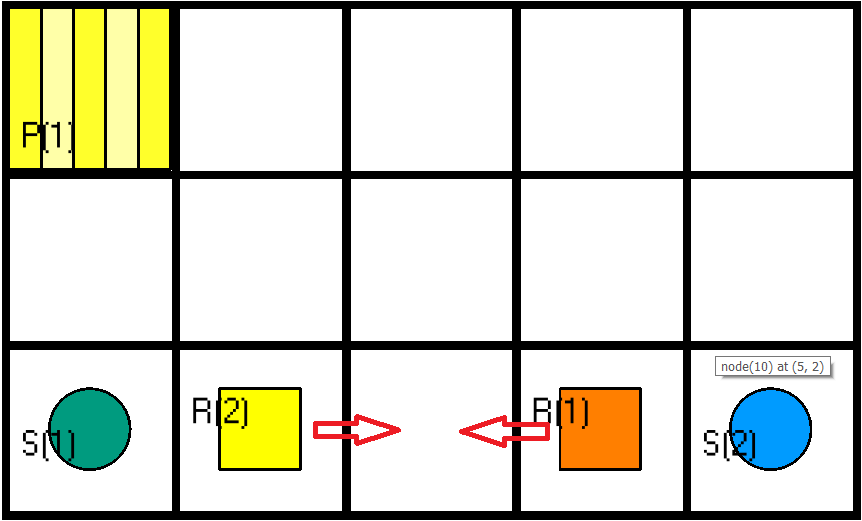
\includegraphics[width=\linewidth]{Images/Conflict 1_1}
   \end{minipage}
   \hspace{.1\linewidth}
   \begin{minipage}[b]{.4\linewidth} 
      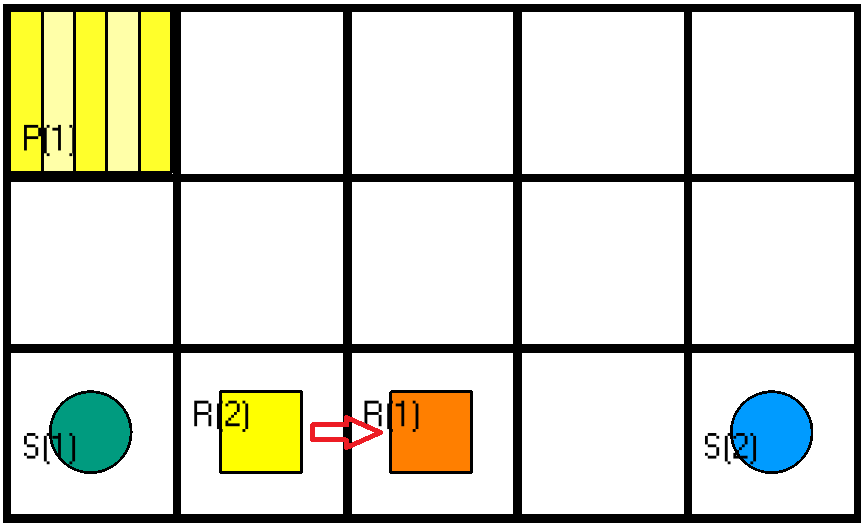
\includegraphics[width=\linewidth]{Images/Conflict 1_2}
   \end{minipage}
\end{figure}
\end{frame}

\begin{frame}
\frametitle{Conflict Detection and Selection}
\begin{figure}
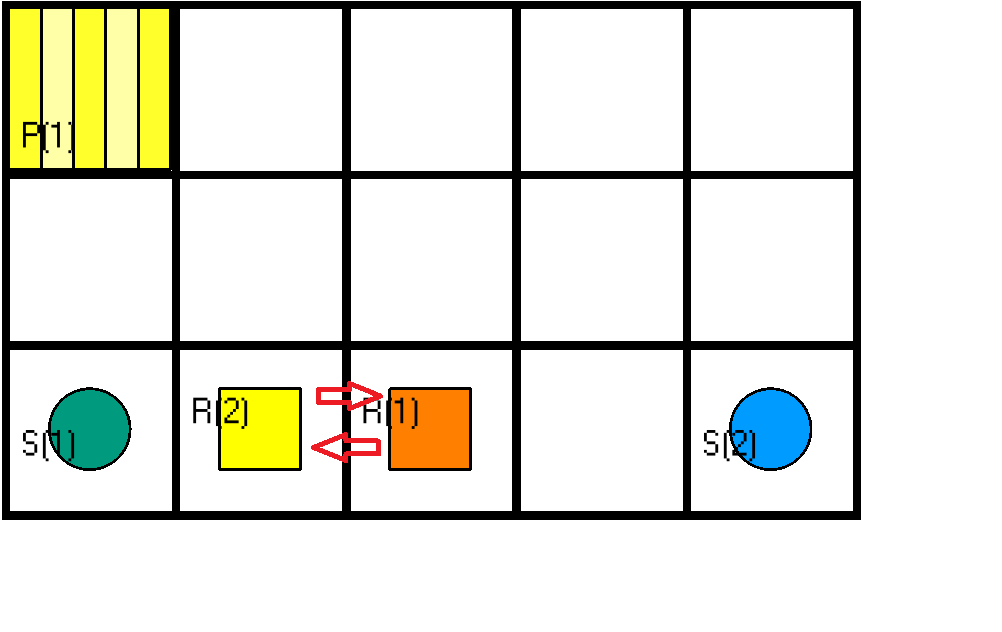
\includegraphics[width=75mm]{Images/Conflict 2}
\end{figure}
\end{frame}


\begin{frame}
\frametitle{Conflict Solving}
\begin{itemize}
\item<2-> Randomly dodge in any possible direction or wait
\item<3-> Wait: remaining plan gets pushed one step back
\item<4-> Dodge: go back at random time step  
\end{itemize}
\end{frame}

\section{Comparison with other Approaches}
\begin{frame}
\frametitle{Unsolvable Benchmarks}
\begin{figure}
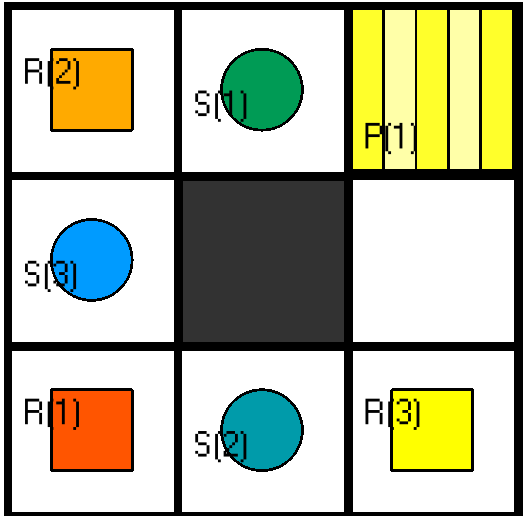
\includegraphics[width=75mm]{Images/Instance 1}
\end{figure}
\end{frame}

\begin{frame}
\frametitle{Unsolvable Benchmarks}
\begin{figure}
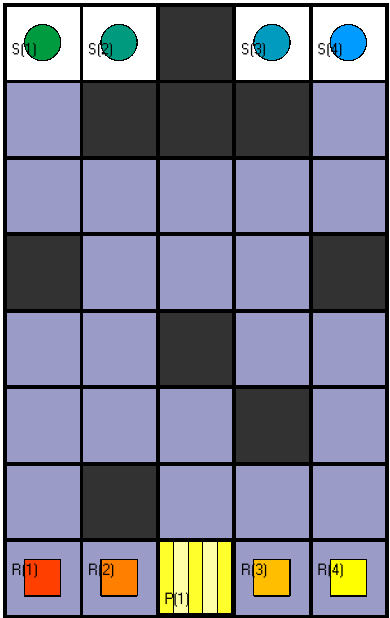
\includegraphics[width=75mm]{Images/Instance 2}
\end{figure}
\end{frame}

\begin{frame}
\frametitle{Unsolvable Benchmarks}
\begin{figure}
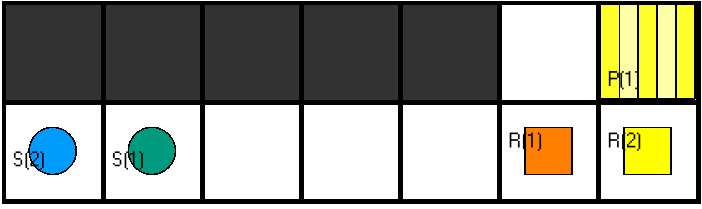
\includegraphics[width=75mm]{Images/Instance 3}
\end{figure}
\end{frame}

\begin{frame}
\frametitle{Comparison with other Approaches}
\begin{itemize}
\item<2-> Very time inefficient
\item<3-> Most other approaches found more efficient solutions
\item<4-> Solves most instances
\item<5-> One other approach better in every way
\end{itemize}
\end{frame}

\section{Conclusion}
\begin{frame}
\frametitle{Conclusion}
\begin{itemize}
\item<2-> Combining plans of single robots
\item<3-> Randomly solve arising conflicts
\item<4-> Time inefficient
\item<5-> Solves most instances
\end{itemize}
\end{frame}

\end{document}